\chapter{Rangkuman Cara Pembuatan Aplikasi Akademik}

\section{Tahapan Pembuatan Aplikasi}
Pada pembuatan aplikasi oracle mahasiswa telah memahami bagaimana cara membuat aplikasi , dengan bantuan data yang ada di microsoft excell.

\begin{enumerate}
\item[1]Buka Microsoft Excell Lalu Kita Membuat data seperti berikut.

\begin{figure}[!htbp]
    \begin{center}
    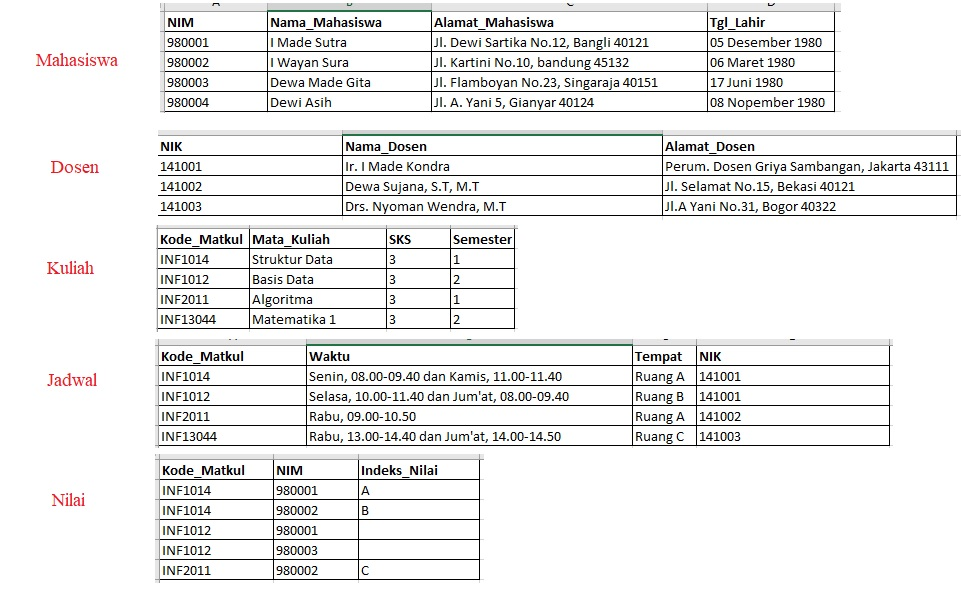
\includegraphics[scale=0.6]{figures/exc.jpg}
    \caption{\textit{Data Excell.}}
    \end{center}   
    \end{figure}
    \par Kita membuat 5 Sheet yaitu Mahasiswa,Dosen,Kuliah,Jadwal,dan Nilai, dalam pembuatan kolom data harus sama, misal NIK berupa angka Semua data pada kolom berarti harus angka, agar bisa terdeteksi oleh sistem Oracle Application Express Tersebut lalu nantinya akan otomatis dibaca oleh sistem.
    \par.

\item[2]Buat Project.
\begin{figure}[!htbp]
    \begin{center}
    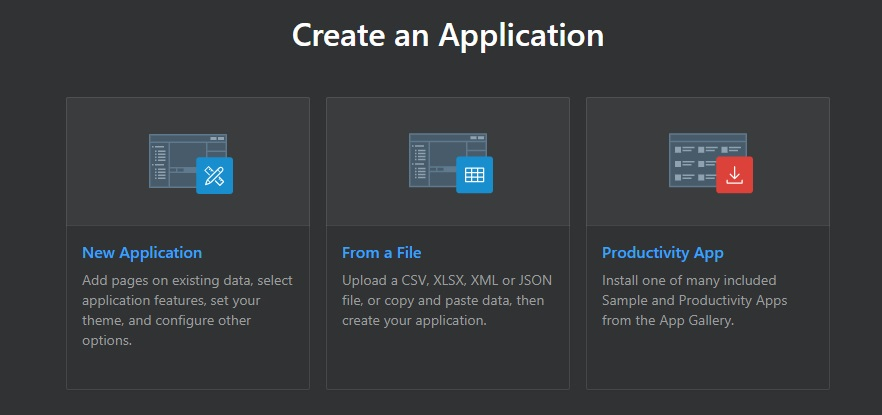
\includegraphics[scale=0.4]{figures/1.jpg}
    \caption{\textit{Halaman Create Application.}}
    \end{center}
\end{figure}
\par Pastikan sudah login lalu masuk pada halaman pembuatan Aplikasi seperti gambar diatas, untuk membukanya Click App Builder lalu pilih Create, pada halaman akan berisi New Application,From A File,dan Productivity App, kita pilih From A File.

\item[3]Pilih File Excell Yang Anda Buat Tadi .
\begin{figure}[!htbp]
    \begin{center}
    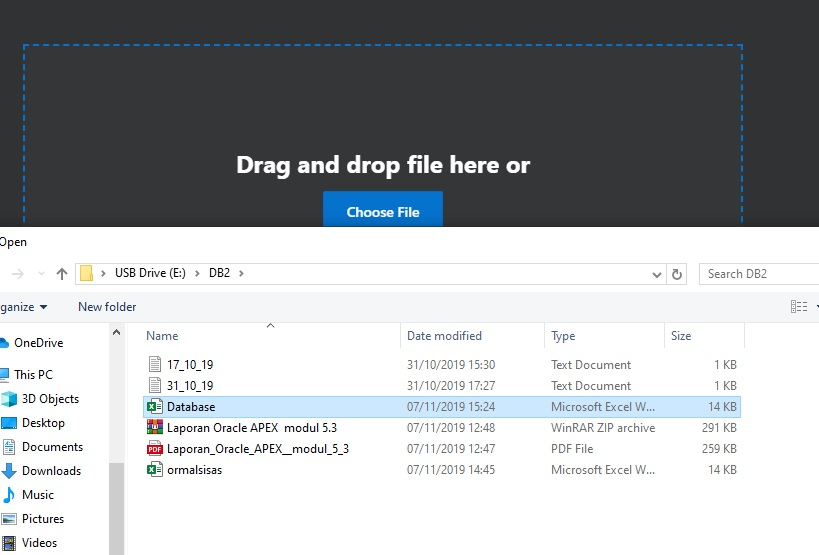
\includegraphics[scale=0.6]{figures/2.jpg}
    \caption{\textit{Open File Excell.}}
    \end{center}
\end{figure}
\par Masukkan file excell anda berupa ekstensi .xlsx lalu klik OK.

\item[4]Memasukkan dan mengatur Tabel .
\begin{figure}[!htbp]
    \begin{center}
    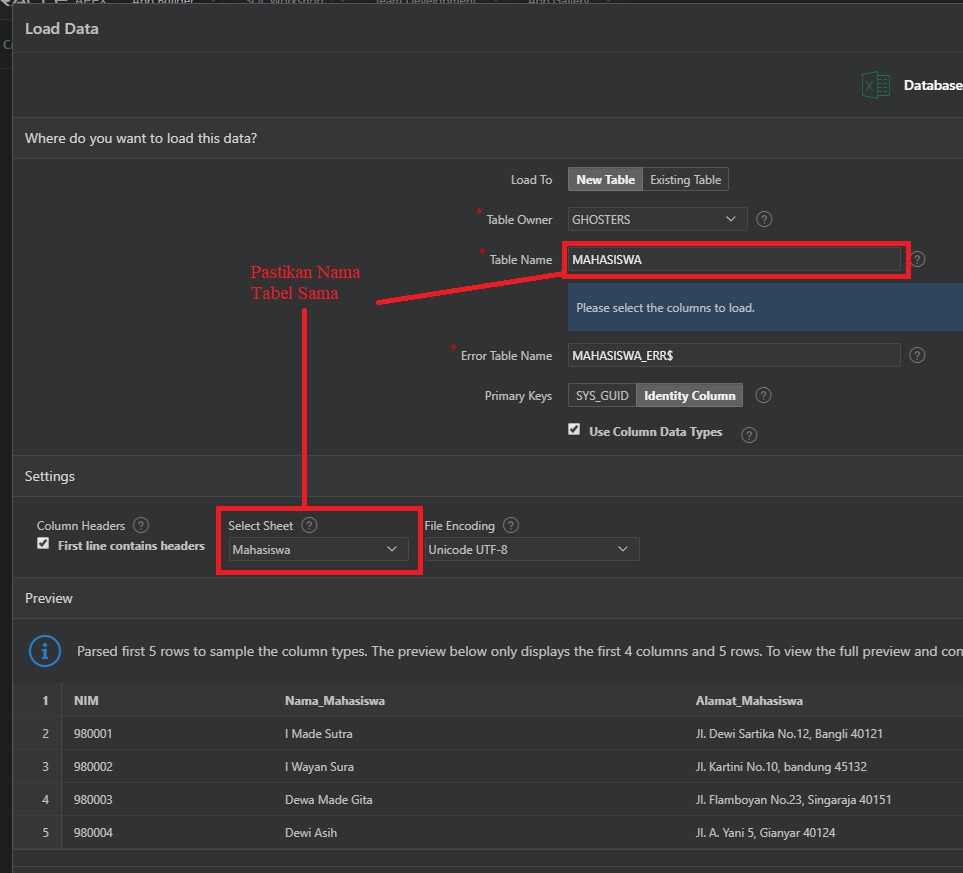
\includegraphics[scale=0.4]{figures/3.jpg}
    \caption{\textit{Pengaturan Tabel.}}
    \end{center}
\end{figure}
\par Setelah itu masuk dalam pengaturan tabel yang akan di Load atau di muat dalam APEX, kita pertama membuat nama tabel Mahasiswa dan pada pengaturan Select Sheet pastikan sama dengan Mahasiswa .

\item[5]Konfigurasi Tabel .
\begin{figure}[!htbp]
    \begin{center}
    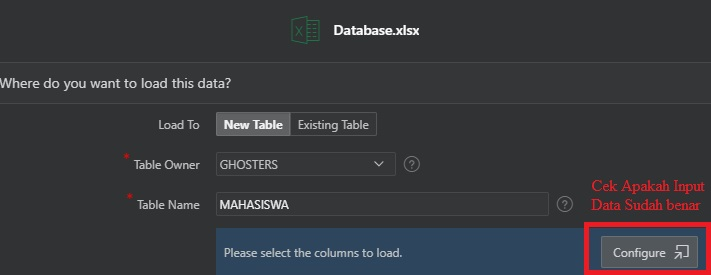
\includegraphics[scale=0.6]{figures/4.jpg}
    \caption{\textit{Konfigurasi Tabel.}}
    \end{center}
\end{figure}
\par Setelah itu masuk dalam konfigurasi tabel yang berisikan tipe data yang valid dalam atribut data, jika ada kesalahan dan segera di perbaiki .

\item[6]Load Data Tabel .
\begin{figure}[!htbp]
    \begin{center}
    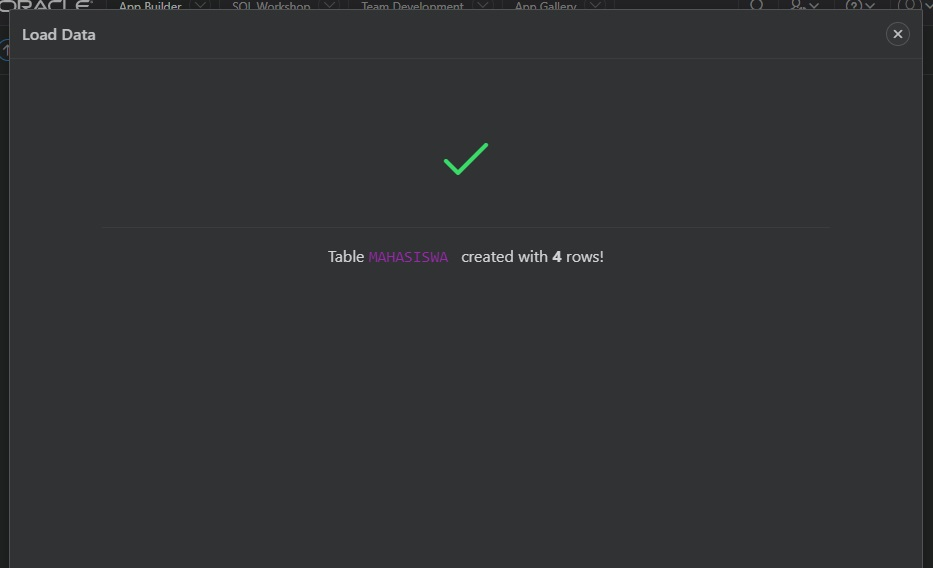
\includegraphics[scale=0.5]{figures/5.jpg}
    \caption{\textit{Load Tabel Sukses.}}
    \end{center}
\end{figure}
\par Setelah itu pencet Load data, dan akan muncul row tabel yang telah dimasukkan tadi, lalu berhenti dahulu dan close, lakukan point ke 3-5 untuk menambahkan tabel Dosen,Kuliah,Jadwal, dan Nilai.

\item[7]Cek Data Tabel .
\begin{figure}[!htbp]
    \begin{center}
    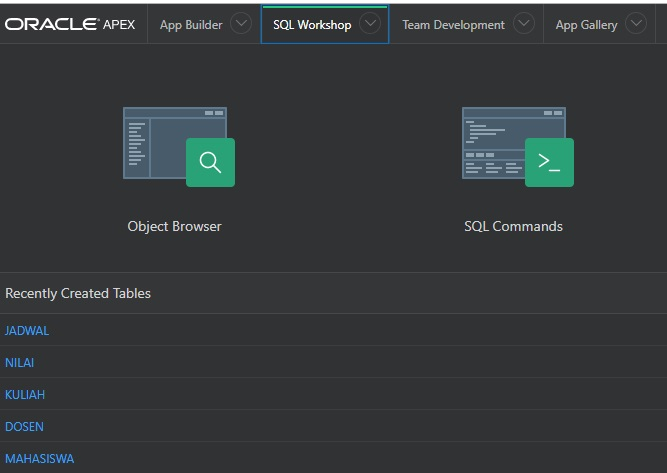
\includegraphics[scale=0.5]{figures/6.jpg}
    \caption{\textit{Cek Tabel.}}
    \end{center}
\end{figure}
\par Cross check dahulu apakah tabel anda sudah terinput seperti gambar ini , lalu cek bagian dalamnya dengan klick nama tabel masing-masing.

\item[8]Cek Tabel Mahasiswa .
\begin{figure}[!htbp]
    \begin{center}
    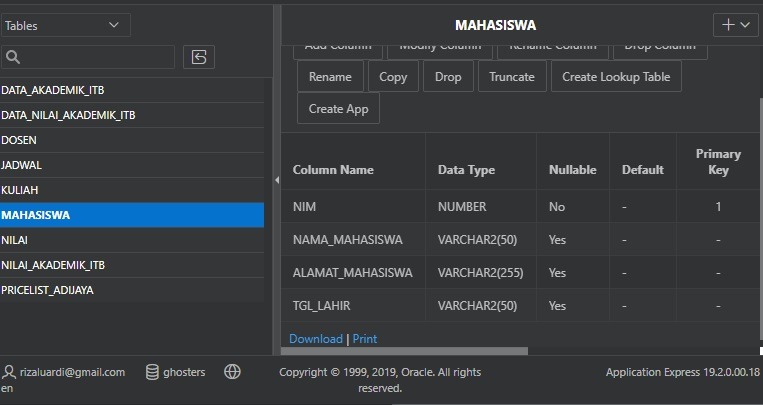
\includegraphics[scale=0.5]{figures/7.jpg}
    \caption{\textit{Cek Tabel Mahasiswa.}}
    \end{center}
\end{figure}
\par Cek terlebih dahulu masing-masing tabel , disini kita ambil contoh tabel mahasiswa.

\item[9]Modifikasi Kolom Tabel .
\begin{figure}[!htbp]
    \begin{center}
    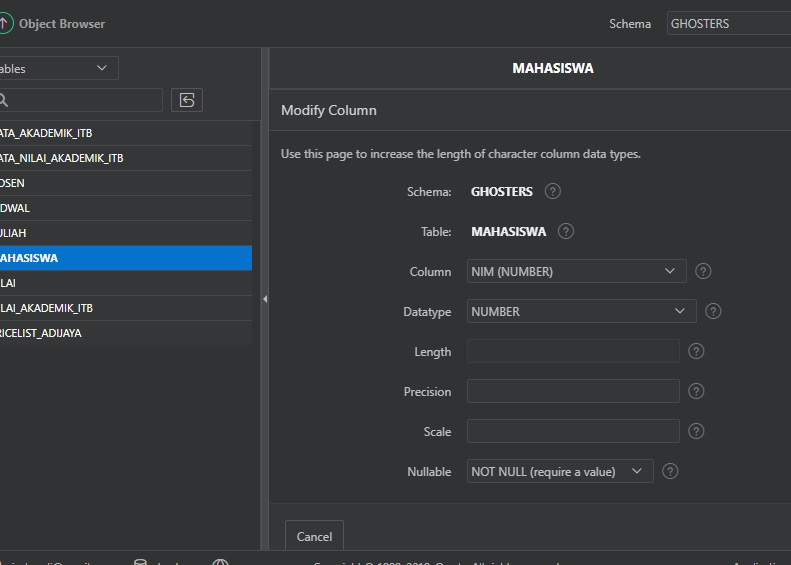
\includegraphics[scale=0.45]{figures/modif_column.jpg}
    \caption{\textit{Memodifikasi Kolom Tabel.}}
    \end{center}
\end{figure}
\par Disini cara untuk memodifikasi kolom jika terdapat satu yang acak-acakan atau data tidak sama anda bisa merubahnya disini seperti contoh mengubah Null menjadi Not Null

\item[10]Menghapus Kolom Tabel .
\begin{figure}[!htbp]
    \begin{center}
    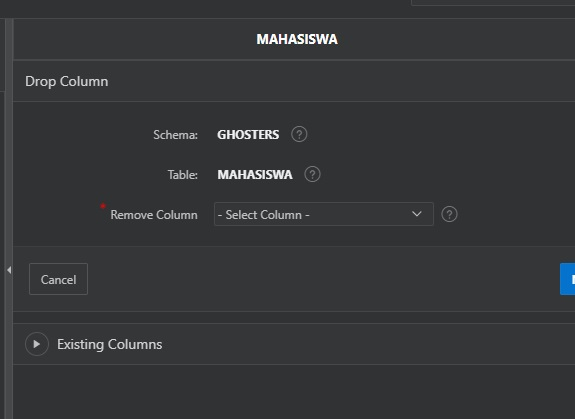
\includegraphics[scale=0.5]{figures/drop_column.jpg}
    \caption{\textit{Menghapus Kolom Tabel.}}
    \end{center}
\end{figure}
\par Disini cara untuk menghapus kolom jika terdapat satu kolom yang tidak sempurna anda bisa menghapusnya.


\item[11]Constraint Kolom Tabel .
\begin{figure}[!htbp]
    \begin{center}
    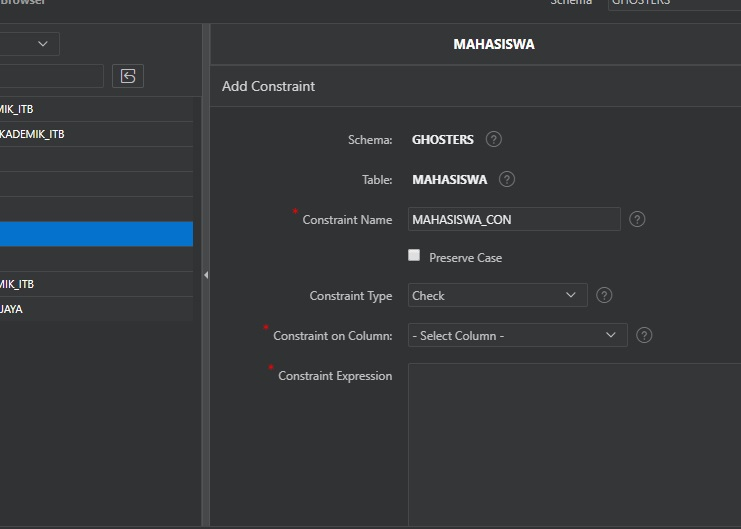
\includegraphics[scale=0.5]{figures/constrainst_column.jpg}
    \caption{\textit{Constraint Kolom Tabel.}}
    \end{center}
\end{figure}
\par Disini cara untuk mengecek, membuat primary key, dan foreign key pada 1 kolom.


\item[12]Menambah Primary Key .
\begin{figure}[!htbp]
    \begin{center}
    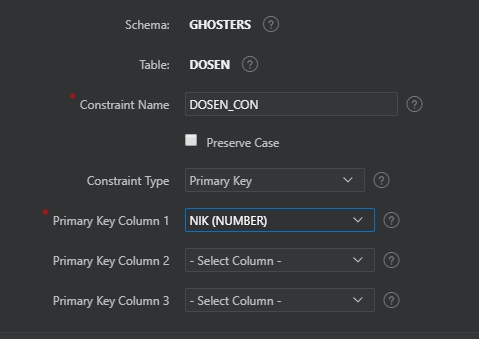
\includegraphics[scale=0.7]{figures/constrainst_column_Pkey.jpg}
    \caption{\textit{Menambah Primary Key.}}
    \end{center}
\end{figure}
\par Disini cara untuk menambah Primary Key sebagai contoh kita merubah pada tabel DOSEN dengan Constraint Name DOSEN CON , lalu tambahkan primary key pada kolom NIK.


\item[13]Menambah Foreign Key .
\begin{figure}[!htbp]
    \begin{center}
    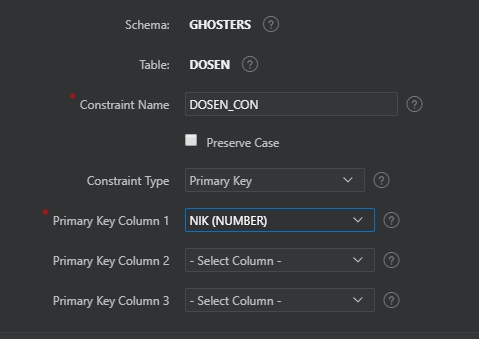
\includegraphics[scale=0.7]{figures/constrainst_column_Pkey.jpg}
    \caption{\textit{Menambah Foreign Key.}}
    \end{center}
\end{figure}
\par Disini cara untuk menambah Foreign key sebagai contoh kita merubah pada tabel NILAI dengan Kolom NIK dan berelasi dengan Tabel MAHASISWA yang ada kolom NIK nya juga dengan cara mengklik NIK yang ada di kiri menuju ke kanan.


\item[14]New Application .
\begin{figure}[!htbp]
    \begin{center}
    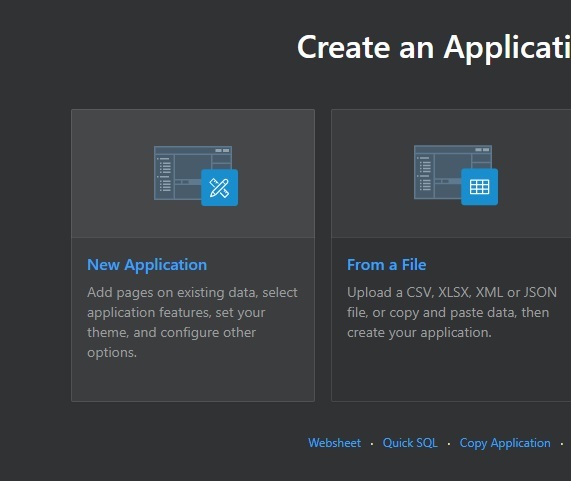
\includegraphics[scale=0.4]{figures/8.jpg}
    \caption{\textit{Menambah Aplikasi.}}
    \end{center}
\end{figure}
\par Setelah semua database dirasa cukup mari kita ke tahap pembuatan aplikasi.


\item[15]Tahapan Membuat Aplikasi 1.
\begin{figure}[!htbp]
    \begin{center}
    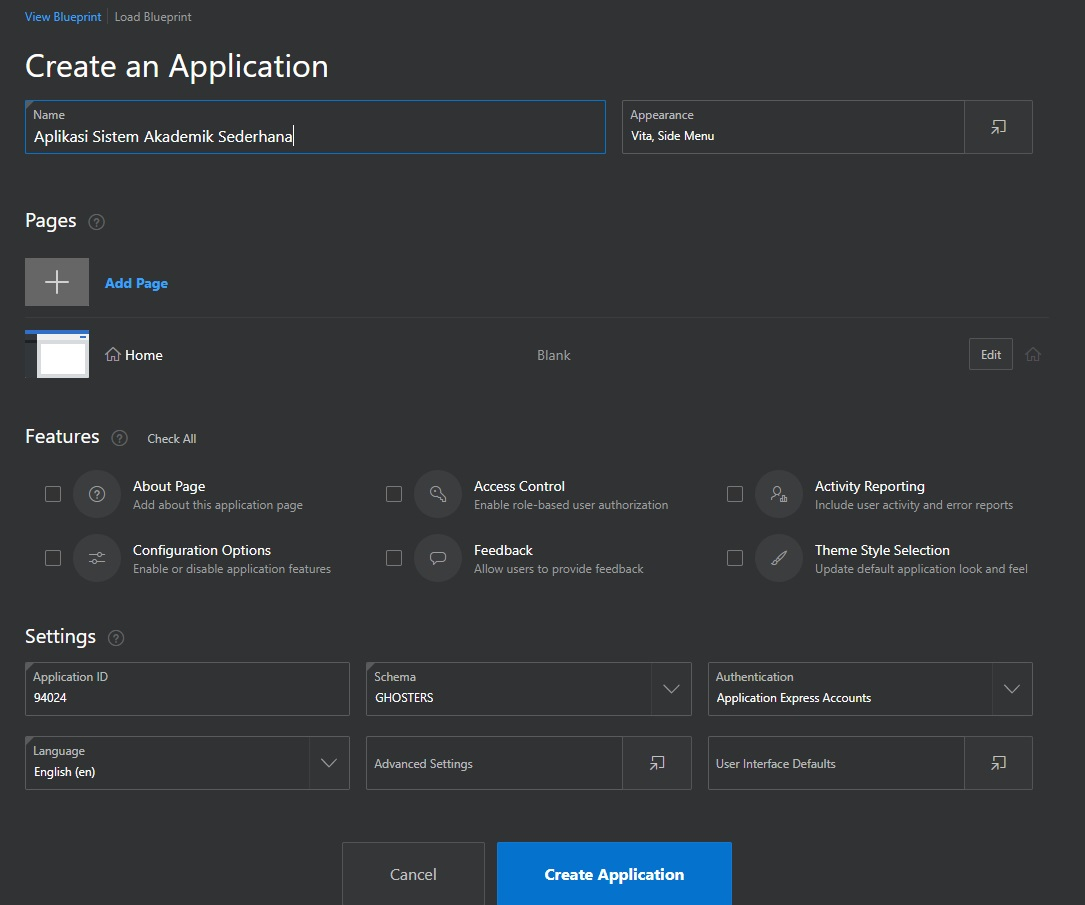
\includegraphics[scale=0.3]{figures/9.jpg}
    \caption{\textit{Tahapan Menambah Aplikasi 1.}}
    \end{center}
\end{figure}
\par Disini sudah akan membuat aplikasi dengan menamai Aplikasi Sistem Akademik Sederhana disana ada Add Page untuk menambah Page, lalu fitur untuk menambah informasi, mari kita check contohnya seperti ini.

\item[16]Add Page .
\begin{figure}[!htbp]
    \begin{center}
    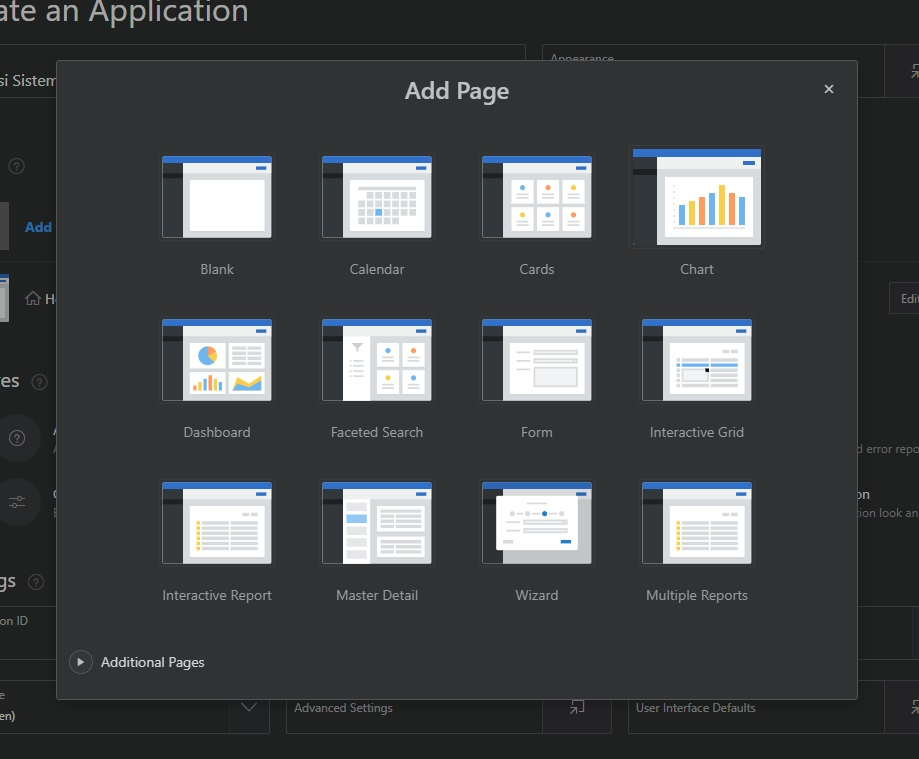
\includegraphics[scale=0.5]{figures/add_page.jpg}
    \caption{\textit{Add Page.}}
    \end{center}
\end{figure}
\par Fitur Add Page dimana untuk menambah page disini tersedia berbagai macam report seperti Interactive Report, Master Detail, Dashboard, dan lain-lain kita ambil contoh Interractive Report dan Master.

\item[17]Interractive Report .
\begin{figure}[!htbp]
    \begin{center}
    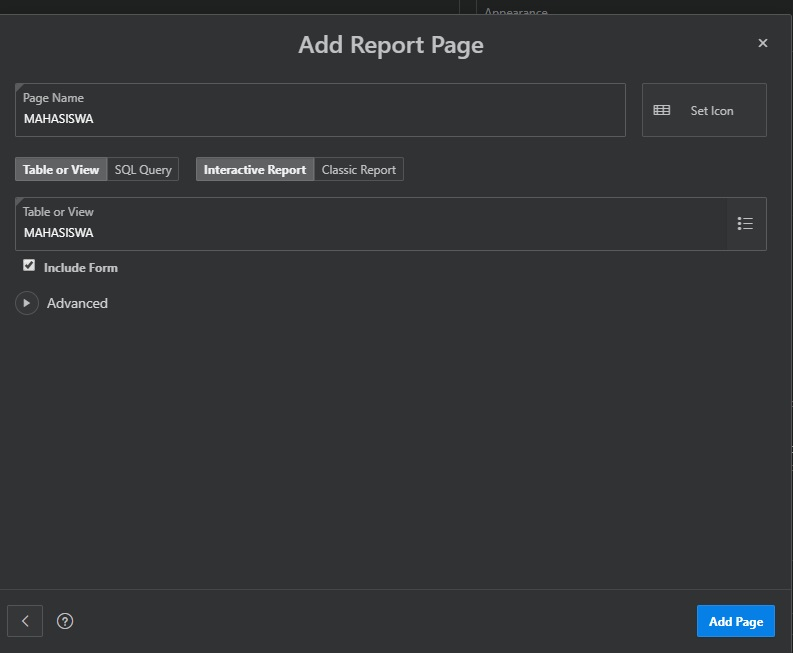
\includegraphics[scale=0.5]{figures/interractive_rprt.jpg}
    \caption{\textit{Interractive Report.}}
    \end{center}
\end{figure}
\par Fitur Interractive report adalah report sederhana yang menunjukkan dari suatu tabel yang akan dipili, caranya sebagai contoh kita akan menambah page MAHASISWA, lalu Table Or View kita ambil dari tabel database MAHASISWA yang kita buat tadi, checkbox Include form untuk menambah Create pada page.

\item[18]Master Detail .
\begin{figure}[!htbp]
    \begin{center}
    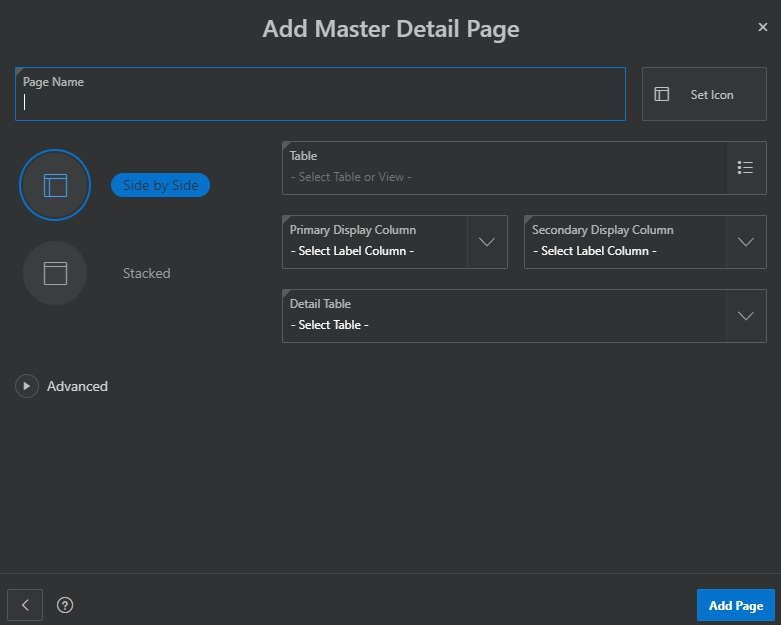
\includegraphics[scale=0.7]{figures/master_dtl.jpg}
    \caption{\textit{MAster Detail.}}
    \end{center}
\end{figure}
\par Pada Master Detail kita beri nama terlebih dahulu, setelah itu pilih tabel yang diinginkan contohnya NILAI , lalu pilih Primary Display Column untuk display pertama, secondary untuk display ke 2 , dan Detail Table untuk menampilkan data jika di klick pada kolom sebelah kanan nanti.

\item[19]Page Yang Dibuat .
\begin{figure}[!htbp]
    \begin{center}
    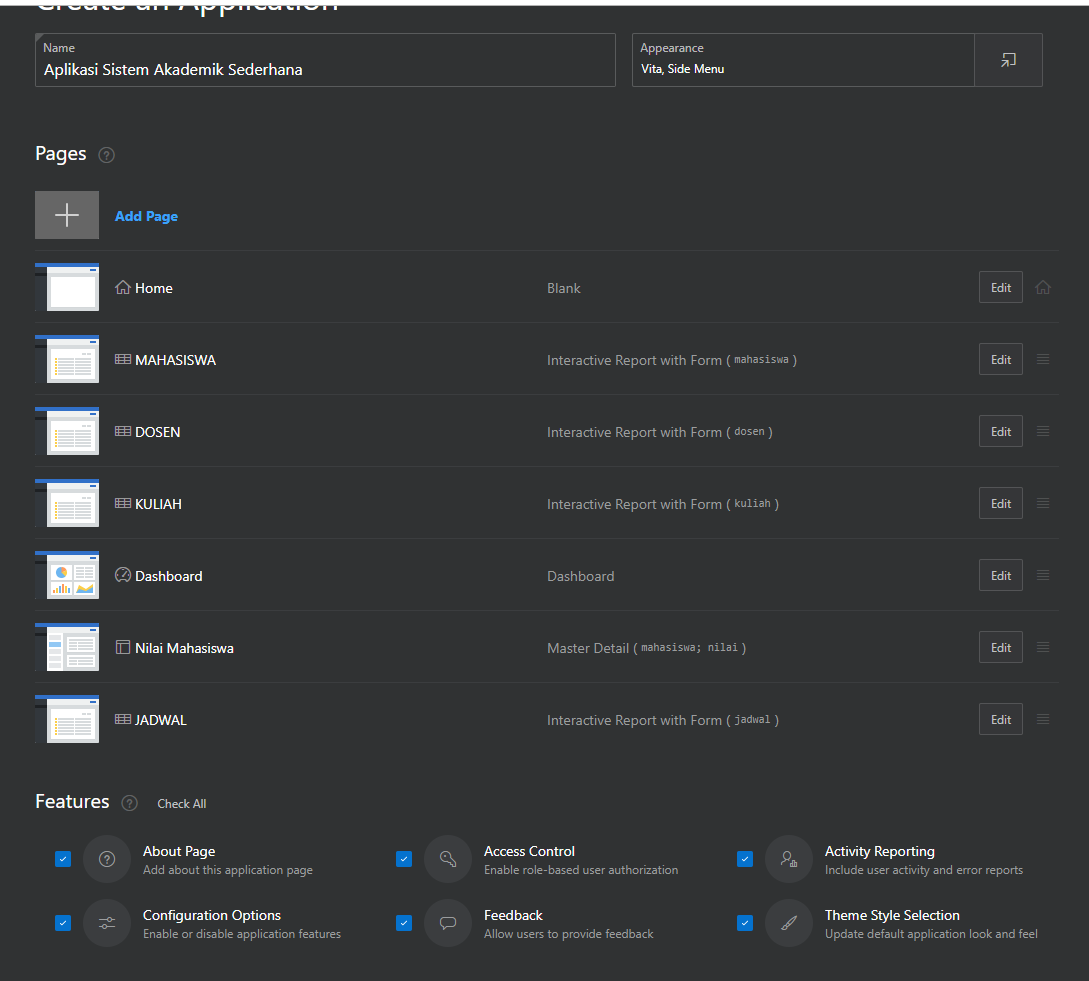
\includegraphics[scale=0.3]{figures/MyApp.png}
    \caption{\textit{Pages Yang Saya Buat.}}
    \end{center}
\end{figure}
\par ini adalah pages dan fitur yang saya buat untuk mempermudah dalam penggunaaannya.

\item[20]Login .
\begin{figure}[!htbp]
    \begin{center}
    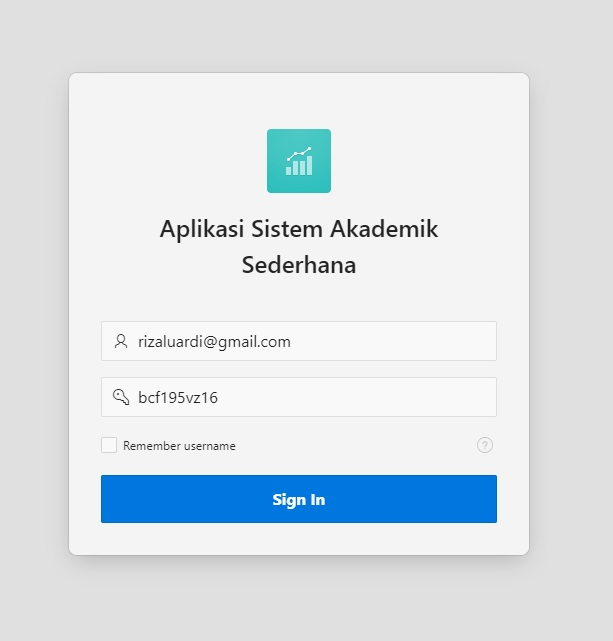
\includegraphics[scale=0.5]{figures/run.jpg}
    \caption{\textit{Login Aplikasi.}}
    \end{center}
\end{figure}
\par https://apex.oracle.com/pls/apex/f?p=94024:1:8341997446025::::: berikut adalah link login apex saya

\item[21]Tampilan Home .
\begin{figure}[!htbp]
    \begin{center}
    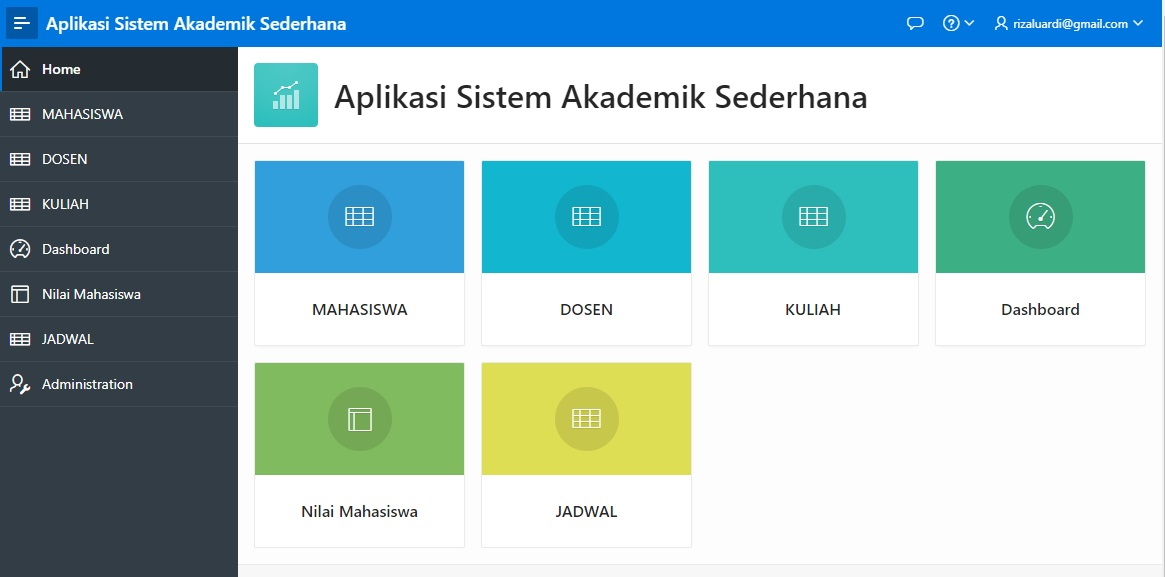
\includegraphics[scale=0.3]{figures/10.jpg}
    \caption{\textit{Tampilan Home.}}
    \end{center}
\end{figure}
\par

\item[22]Tampilan Mahasiswa .
\begin{figure}[!htbp]
    \begin{center}
    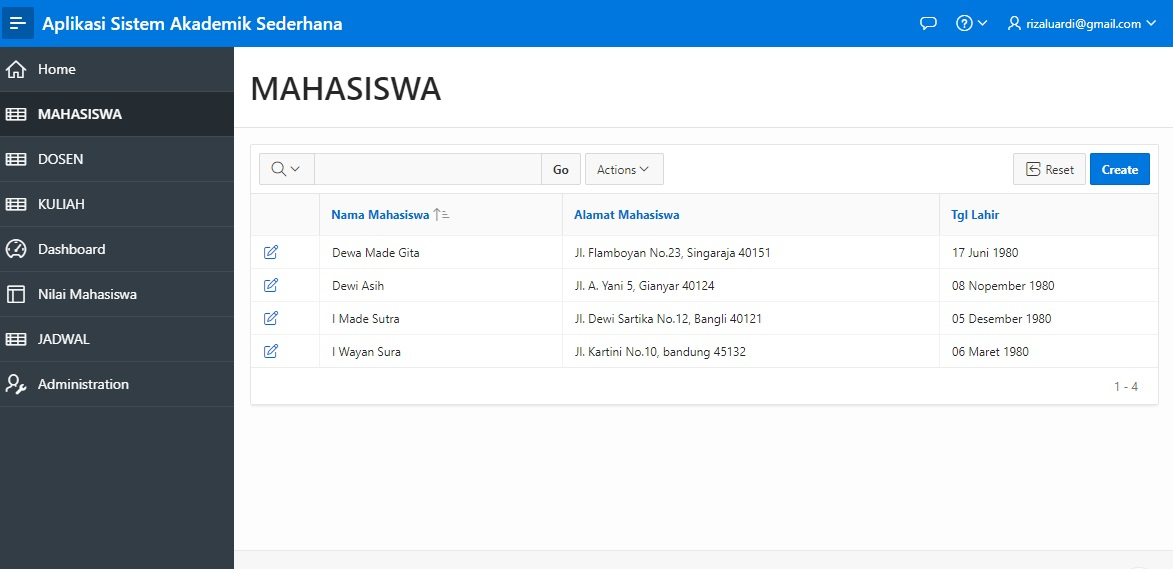
\includegraphics[scale=0.3]{figures/mhs.jpg}
    \caption{\textit{Tampilan Home.}}
    \end{center}
\end{figure}
\par

\item[23]Tampilan Dosen .
\begin{figure}[!htbp]
    \begin{center}
    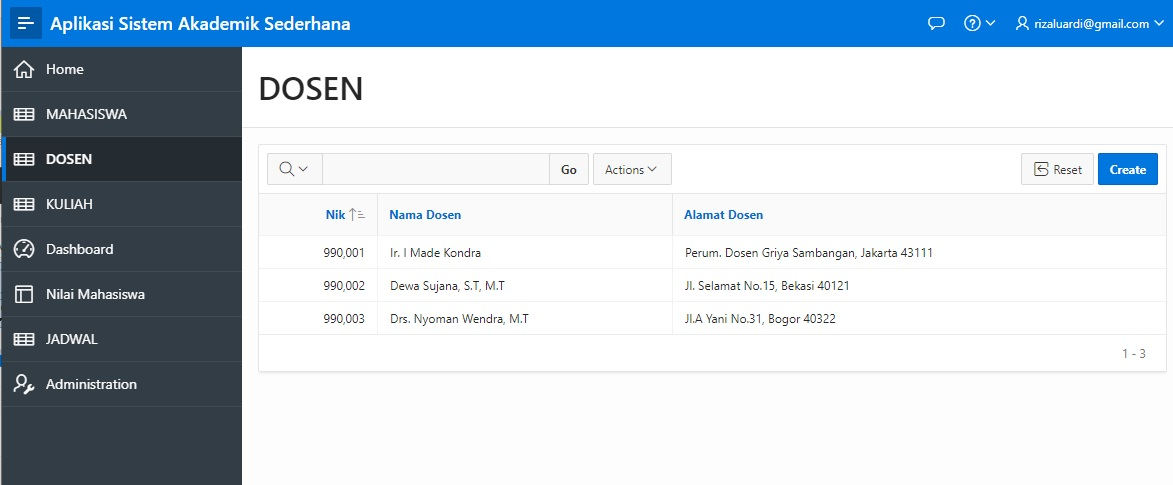
\includegraphics[scale=0.3]{figures/dsn.jpg}
    \caption{\textit{Tampilan Dosen.}}
    \end{center}
\end{figure}
\par

\item[24]Tampilan Kuliah .
\begin{figure}[!htbp]
    \begin{center}
    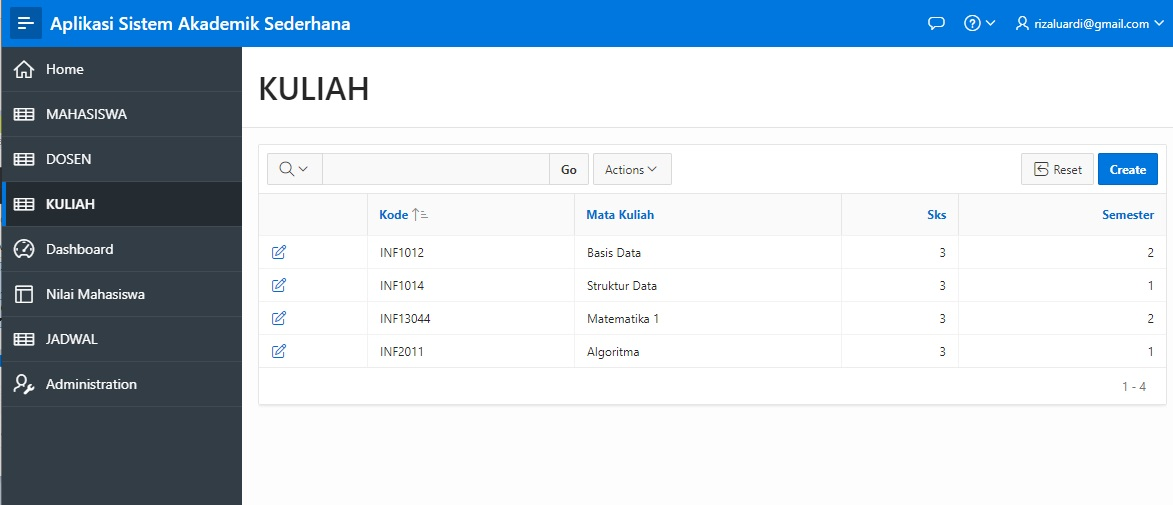
\includegraphics[scale=0.3]{figures/klh.jpg}
    \caption{\textit{Tampilan Kuliah.}}
    \end{center}
\end{figure}
\par

\item[25]Tampilan Nilai Mahasiswa .
\begin{figure}[!htbp]
    \begin{center}
    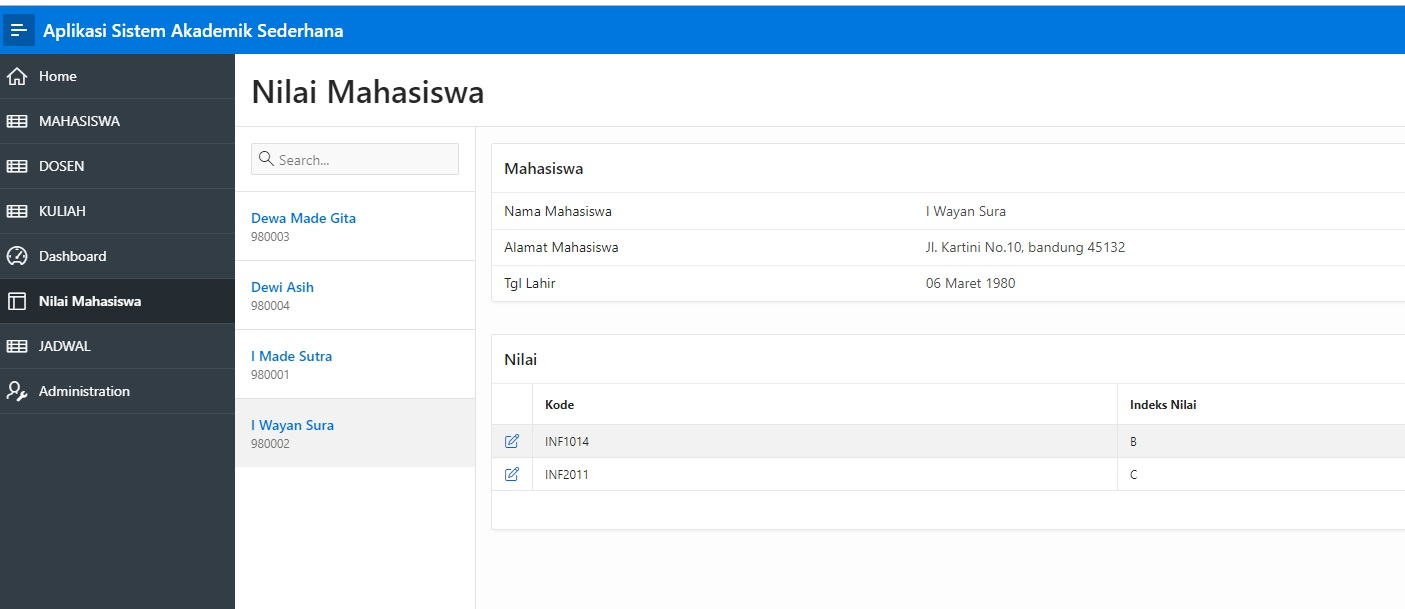
\includegraphics[scale=0.3]{figures/nilaimhs.jpg}
    \caption{\textit{Tampilan Mahasiswa.}}
    \end{center}
\end{figure}
\par

\item[26]Tampilan Dasbor .
\begin{figure}[!htbp]
    \begin{center}
    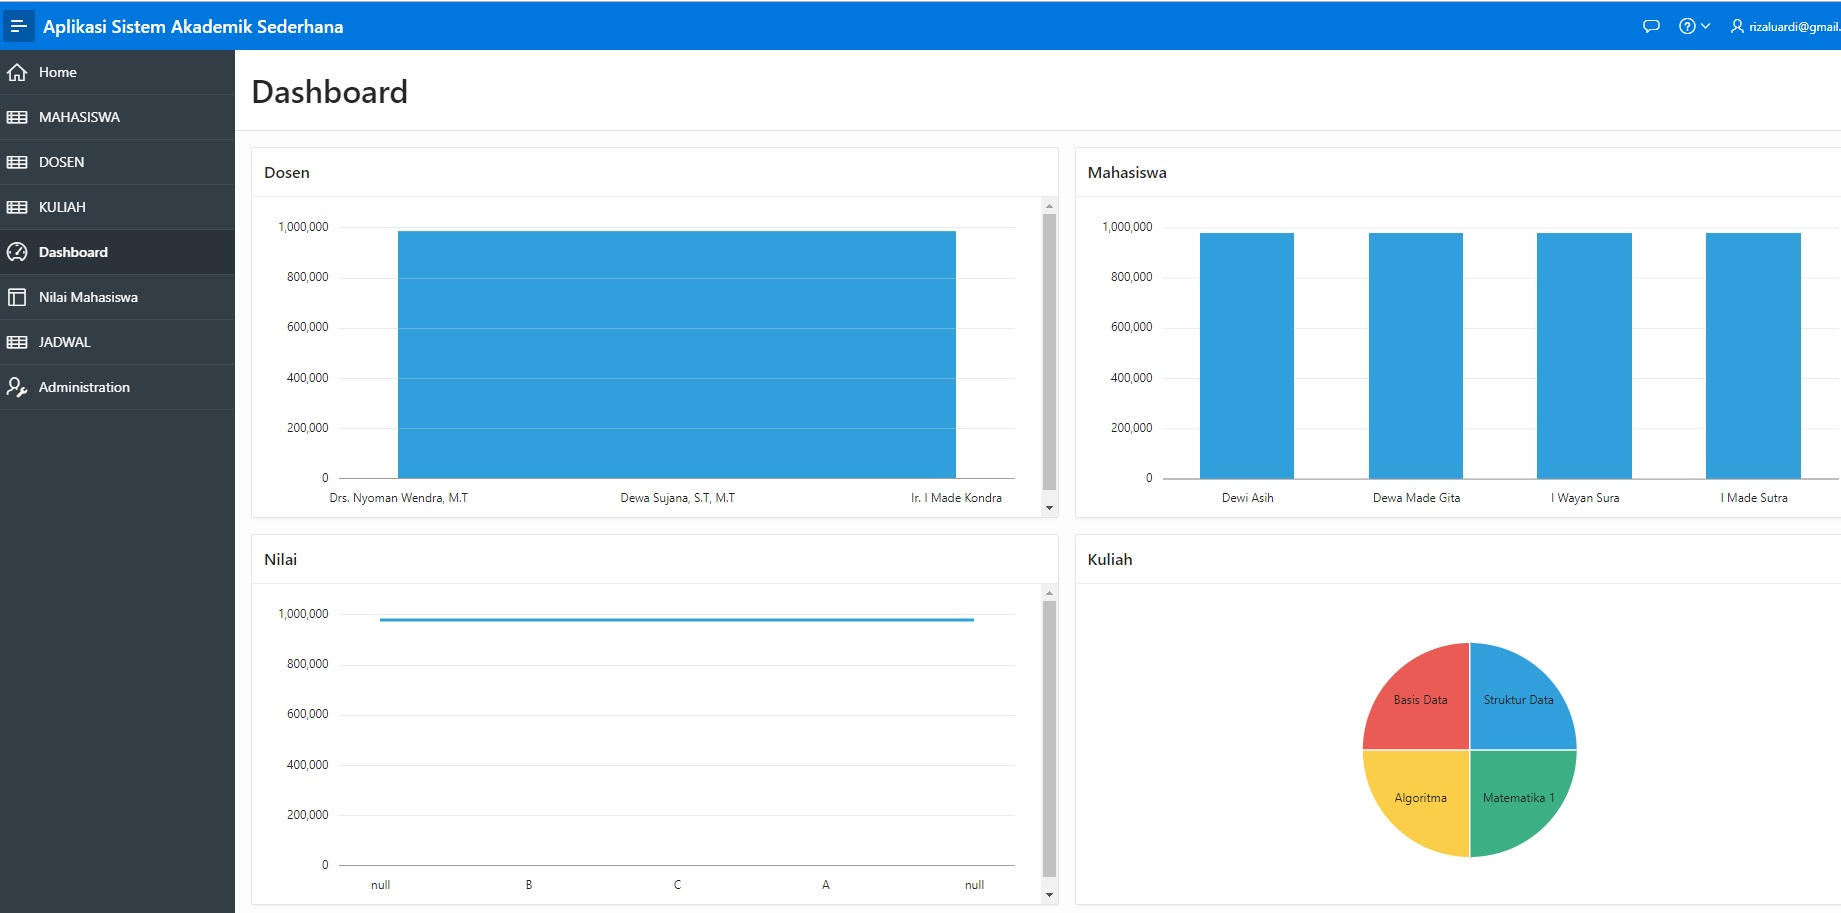
\includegraphics[scale=0.2]{figures/dasbor.jpg}
    \caption{\textit{Tampilan Dasbor.}}
    \end{center}
\end{figure}
\par

\item[27]Tampilan Jadwal .
\begin{figure}[!htbp]
    \begin{center}
    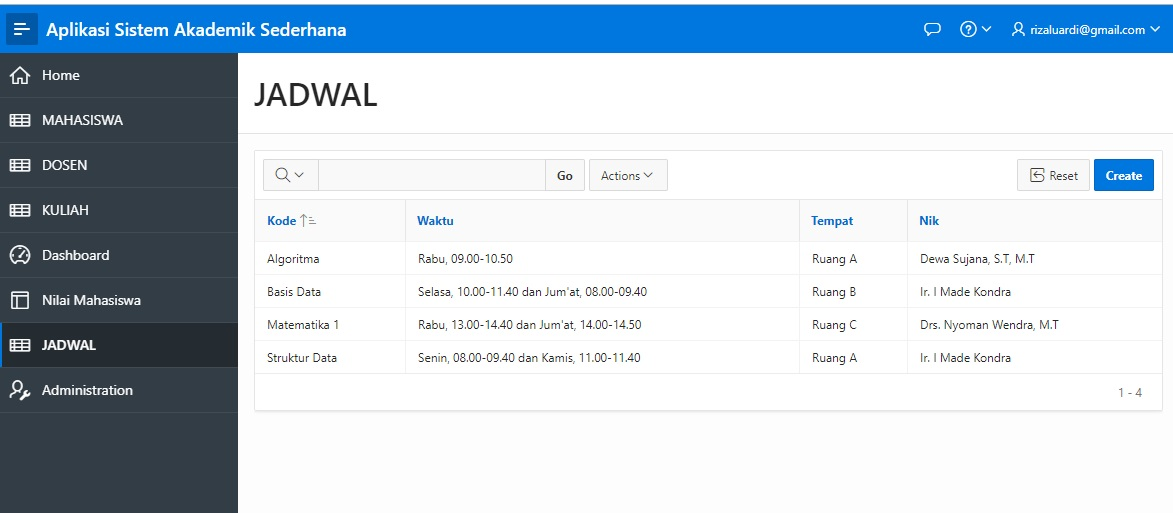
\includegraphics[scale=0.3]{figures/jadwal.jpg}
    \caption{\textit{Tampilan Jadwal.}}
    \end{center}
\end{figure}
\par
\end{enumerate}
